\chapter{\texorpdfstring{Diagnosis for Workflow Nets}{Diagnosis for Workflow Nets}}
\label{ch:21}
\lecturemeta{Lezione 21 \quad\textbullet\quad 2026-07-04 \quad\textbullet\quad Roberto Bruni}{van der Aalst, \emph{Diagnosing workflow processes using Woflan} (articolo, opzionale)}

Sappiamo ormai \textbf{verificare} se un workflow net è sound (liveness + boundedness di $N^\star$, \hyperref[ch:12]{12 — Soundness}) e conosciamo classi di reti — \hyperref[ch:15]{S-net/T-net}, \hyperref[ch:17]{free-choice} — dove questa verifica è più semplice o addirittura strutturale. L'ultima lezione del corso completa il quadro con l'altra metà del problema: quando un net \textbf{non} è sound, come lo \textbf{diagnostichiamo}? Non basta un verdetto "non sound" — un progettista ha bisogno di sapere \textbf{dove} e \textbf{perché}. Vedremo tre strumenti, dal più strutturale (S-coverability) al più comportamentale (error sequences), così come implementati in tool reali (WoPeD, Woflan).

\section{\texorpdfstring{S-coverability: certificare l'S-invariant positivo "a pezzi"}{S-coverability: certificare l'S-invariant positivo "a pezzi"}}

Ricordiamo il \hyperref[ch:17]{Rank Theorem}: un free-choice system è live e bounded sse valgono sei condizioni, fra cui "\emph{ha un S-invariant positivo}". Il problema pratico è: \textbf{come si trova} un tale invariante, in modo intuitivo e non solo risolvendo un sistema lineare?

\begin{boxtip}{L'idea: decomporre in filoni paralleli}
Un caso reale è spesso composto da \textbf{filoni di controllo paralleli} (thread), ciascuno dei quali impone un ordine sui propri task. L'idea è decomporre la rete in \textbf{sotto-reti S-net} (una per filone) tali che \textbf{ogni place} della rete appartenga ad almeno una di esse (un place può comparire in più filoni). Ogni S-net induce, come sappiamo da \hyperref[ch:15]{15 — S-T Systems}, un \textbf{S-invariant uniforme}; sommandoli si ottiene un \textbf{S-invariant positivo} sull'intera rete.
\end{boxtip}

Per formalizzare "sotto-rete S-net che si comporta bene", serve prima il concetto generale di \textbf{sottorete}, poi la nozione più specifica di \textbf{S-component}.

\begin{boxdefinition}{Subnet}
Dato $N=(P,T,F)$ e un insieme di nodi $X \subseteq P \cup T$, la \textbf{subnet} indotta da $X$ è $N' = (P\cap X,\, T\cap X,\, F\cap(X\times X))$: si prende un sottoinsieme di nodi e si \textbf{dimenticano} tutti gli archi verso l'esterno.
\end{boxdefinition}

\begin{boxdefinition}{S-component}
Una subnet $N'$ indotta da $X$ è un \textbf{S-component} se: 1. è uno \textbf{S-net strongly connected} (\hyperref[ch:15]{S-net}: ogni transizione ha esattamente un place in ingresso e uno in uscita); 2. per ogni place $p \in X \cap P$, \textbf{tutte} le transizioni collegate a $p$ (sia $\bullet p$ sia $p\bullet$) sono in $X$ — "se prendi un place, devi prendere anche tutte le sue transizioni".

La condizione 2 è cruciale: evita di "tagliare a metà" le scelte di un place, garantendo che la subnet catturi \emph{fedelmente} il comportamento locale di quel filone.
\end{boxdefinition}

\begin{figure}[!htb]
\centering
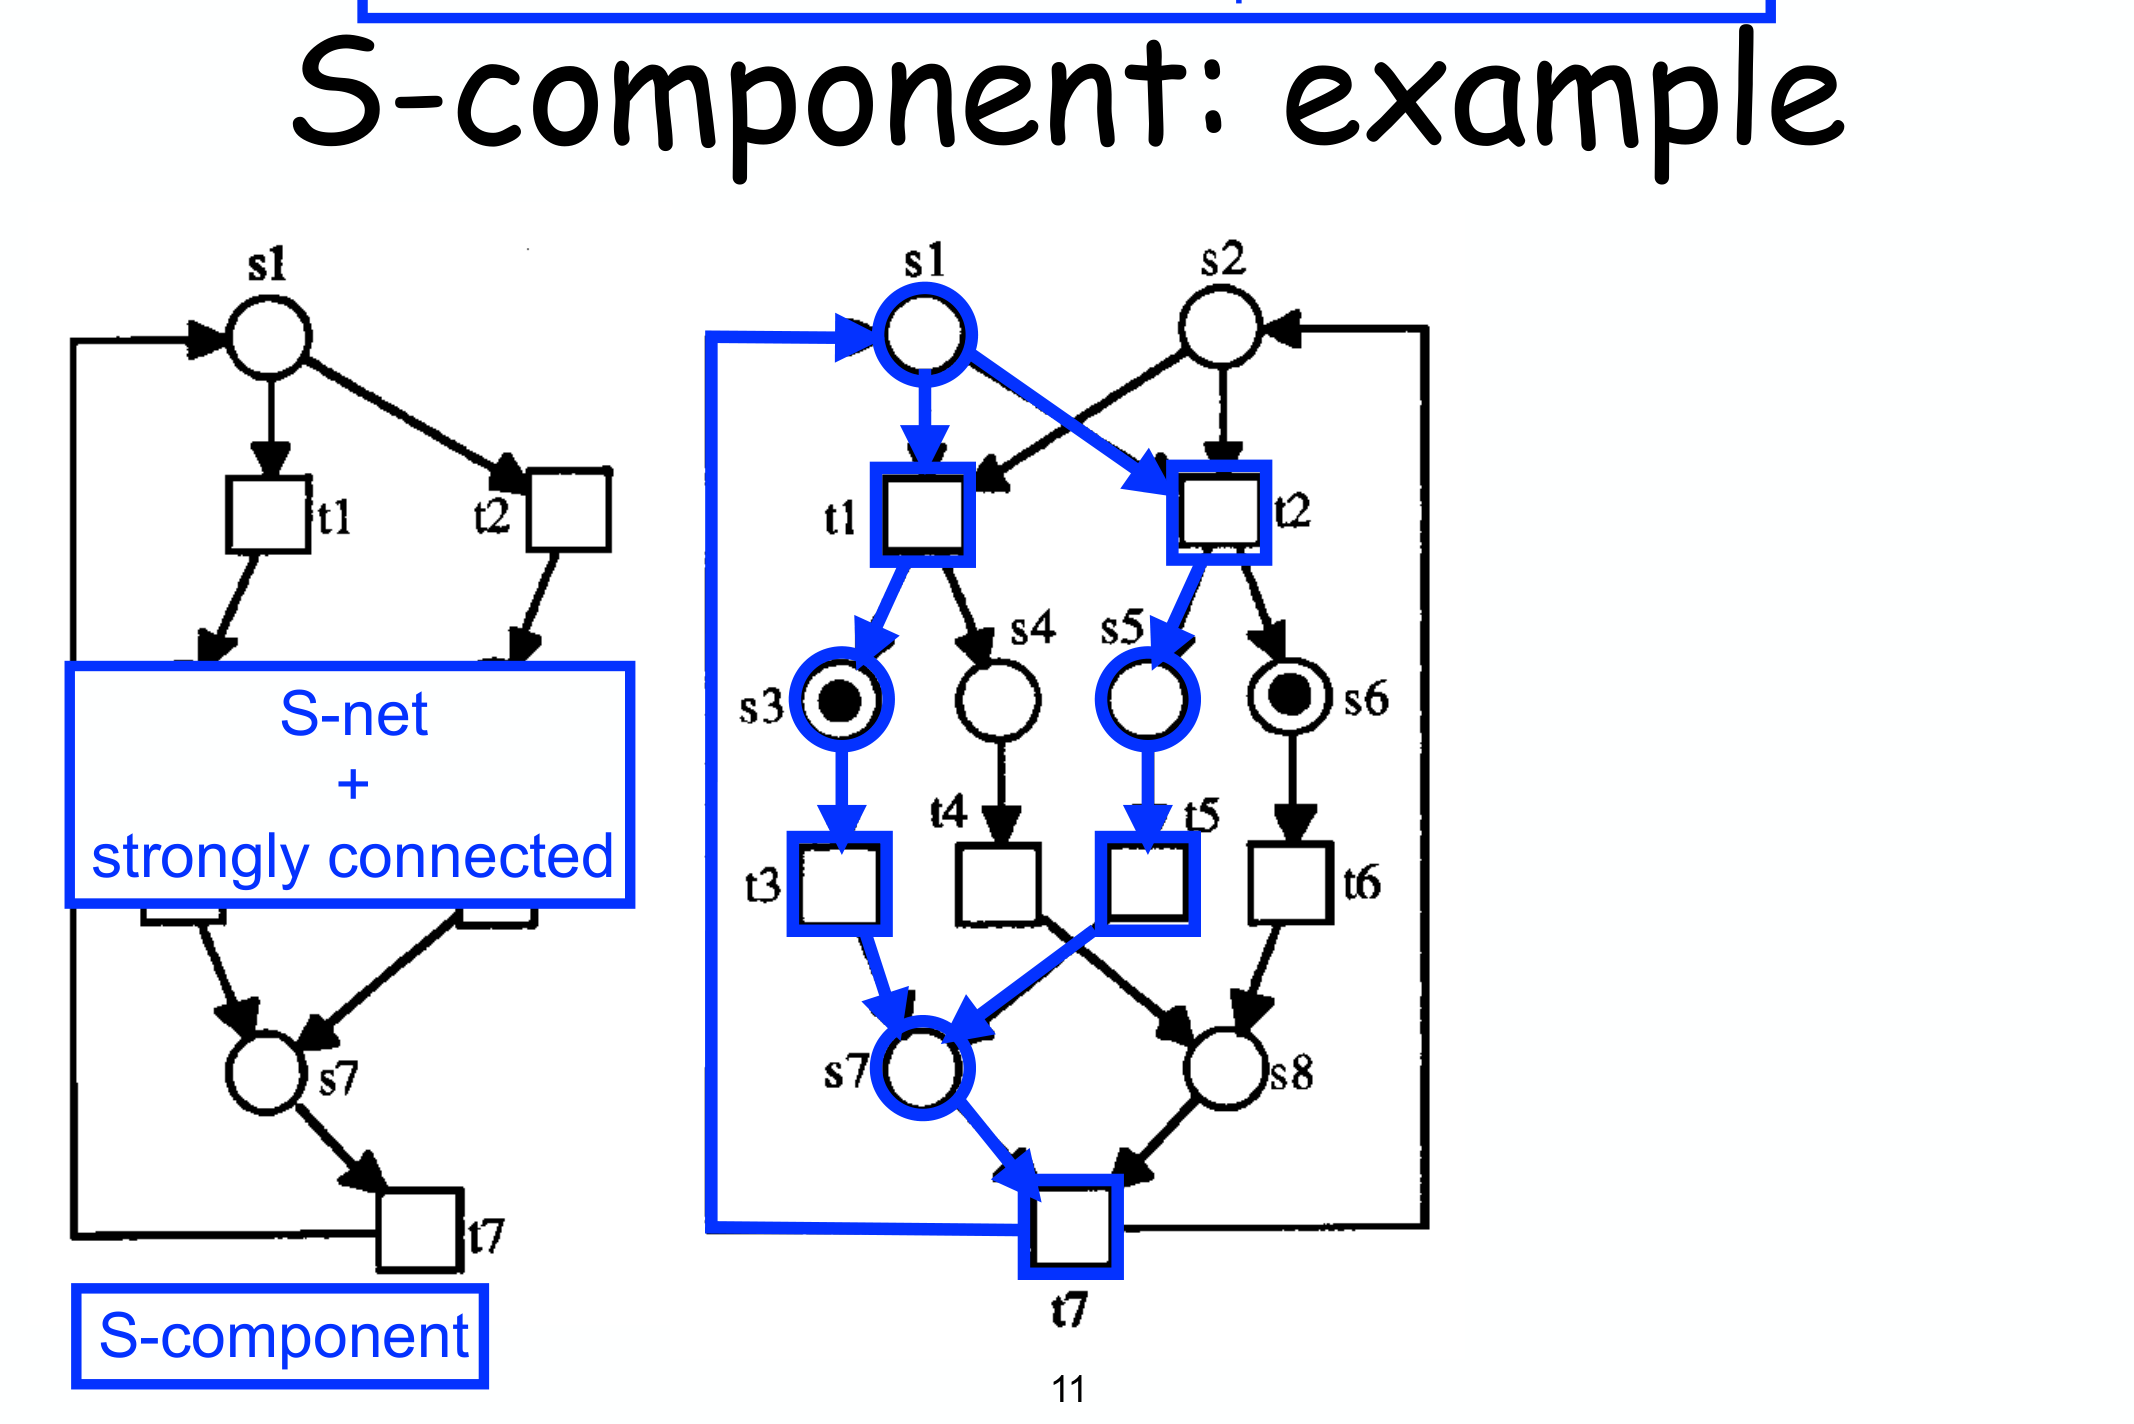
\includegraphics[width=0.74\linewidth,height=0.34\textheight,keepaspectratio]{images/21-wfnets-diagnosis_p11_s-component-example.png}
\caption{Un S-component (in blu): un ciclo \textbf{S-net strongly connected} dove, per ogni place incluso, \textbf{tutte} le transizioni ad esso collegate sono incluse a loro volta — altrimenti non sarebbe un S-net valido (si perderebbe l'alternanza "un solo arco in ingresso/uscita per transizione").}
\end{figure}

Un solo S-component copre solo \emph{alcuni} place; per coprirli tutti serve una \textbf{collezione}.

\begin{boxdefinition}{S-cover}
Un \textbf{S-cover} di $N$ è un insieme $C$ di S-component tale che \textbf{ogni place} di $N$ appartenga ad almeno uno di essi. $N$ è \textbf{S-coverable} se ammette un S-cover.
\end{boxdefinition}

\begin{figure}[!htb]
\centering
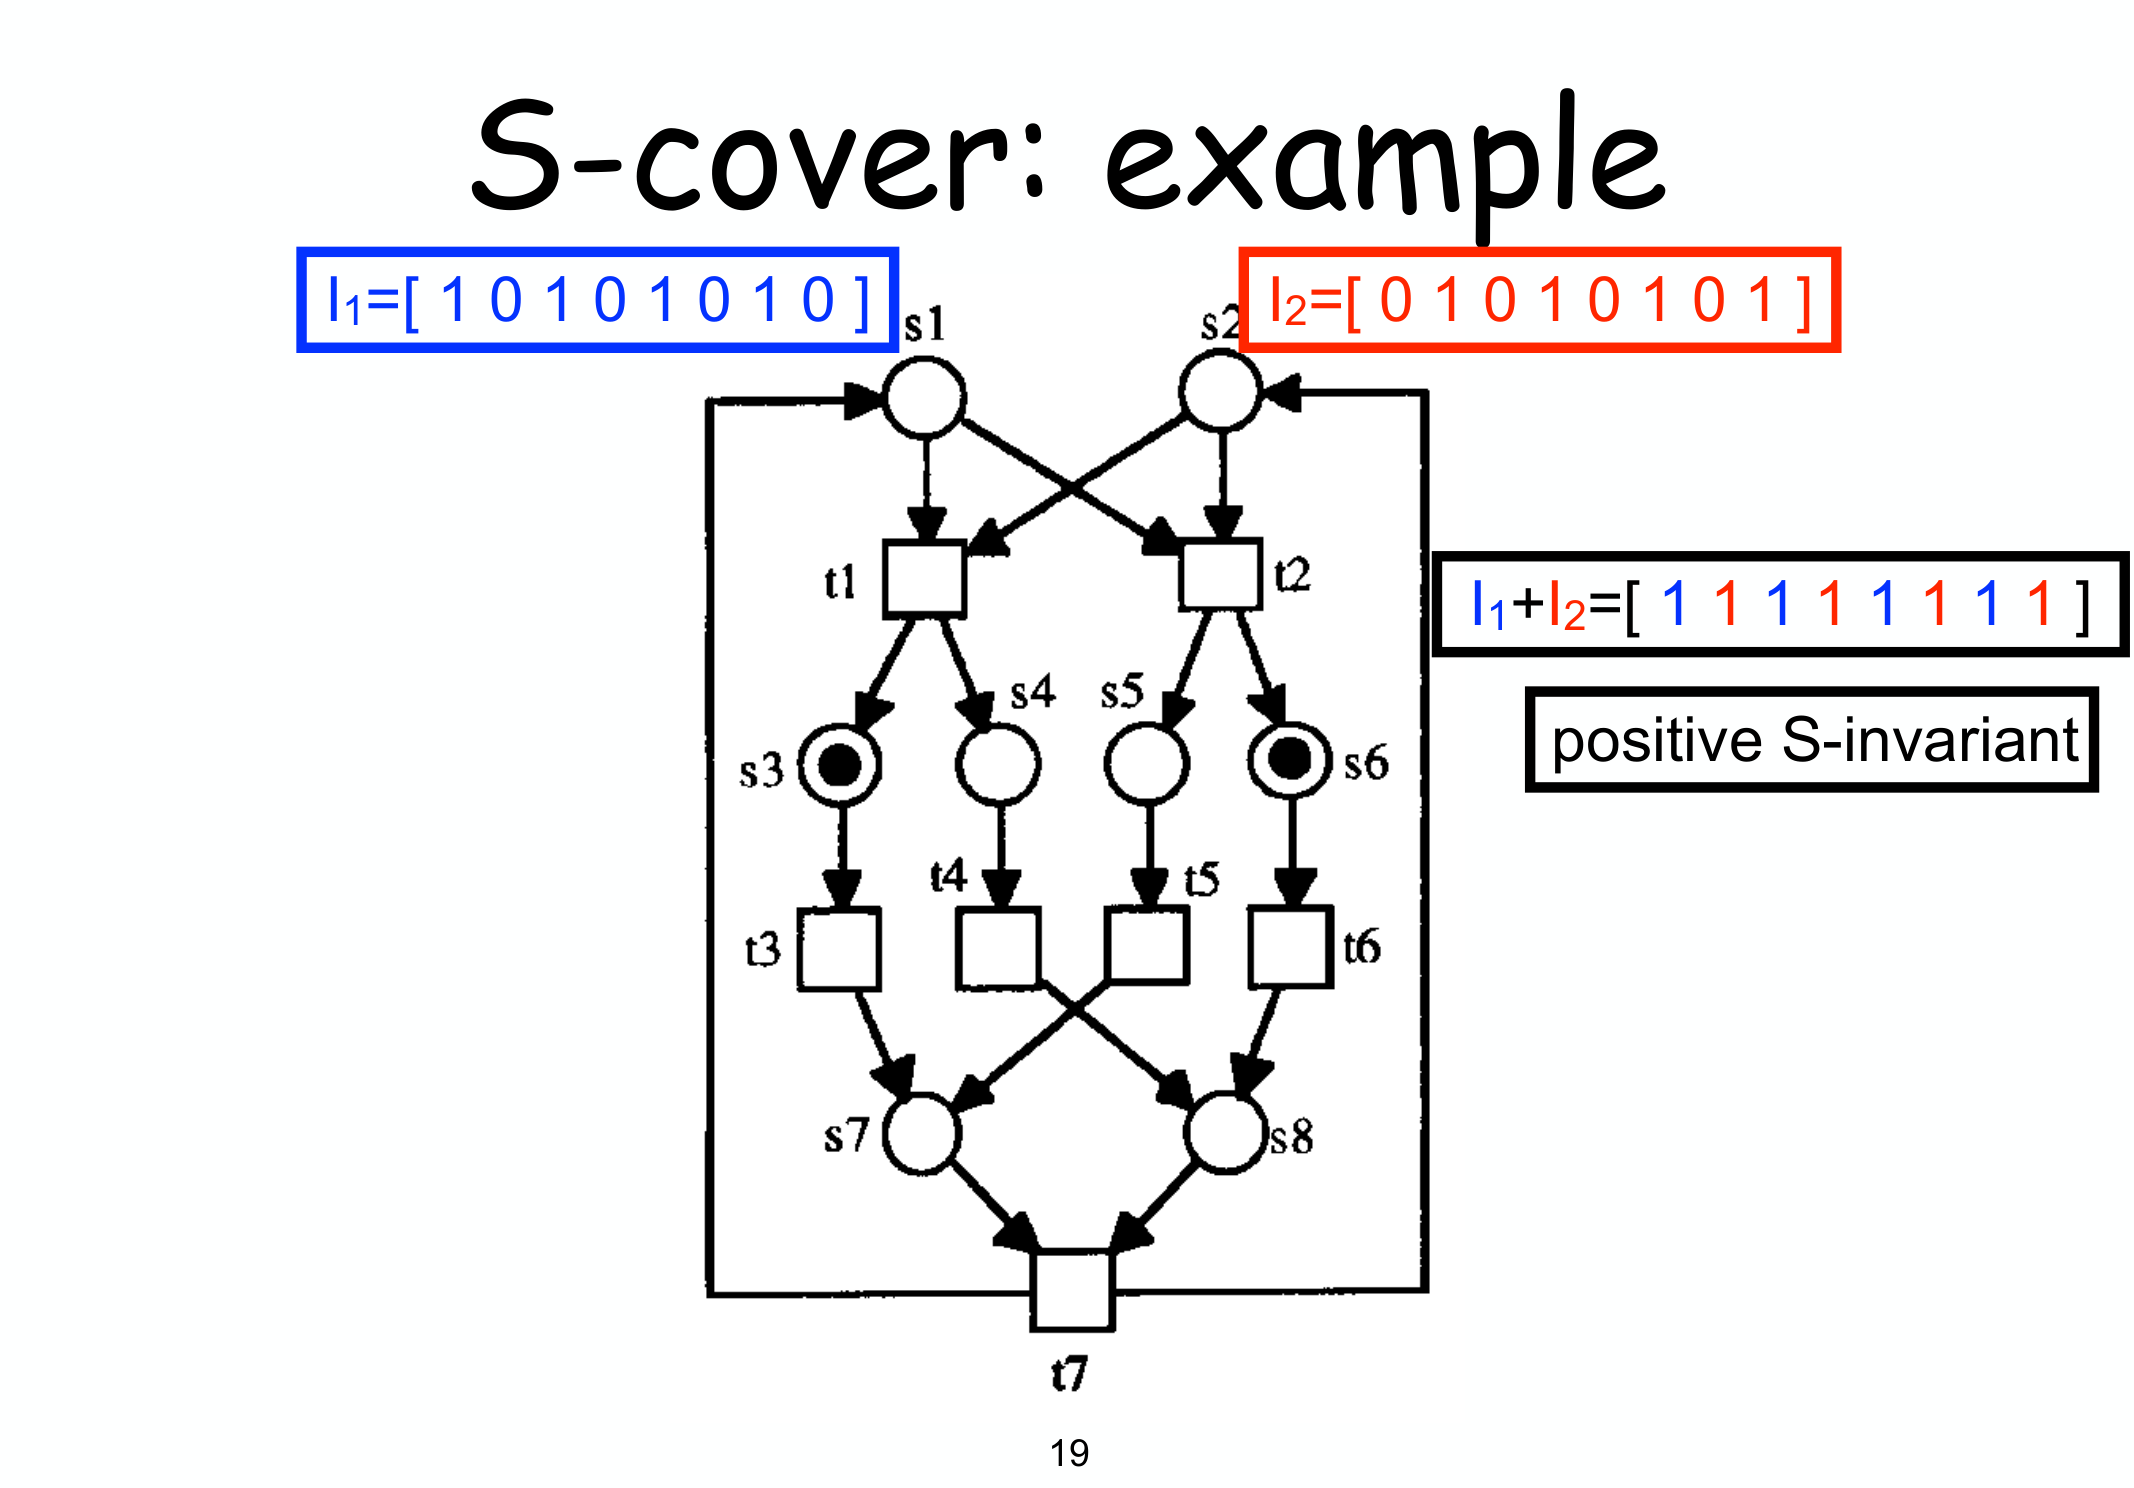
\includegraphics[width=0.74\linewidth,height=0.34\textheight,keepaspectratio]{images/21-wfnets-diagnosis_p19_s-cover-example.png}
\caption{Un S-cover con due S-component. Ciascuno induce un S-invariant uniforme (peso 1 sui place coperti, 0 altrove); \textbf{sommandoli} ($I_1+I_2$) si ottiene un S-invariant \textbf{positivo} su tutta la rete — la ricetta pratica per certificare uno dei sei ingredienti del Rank Theorem.}
\end{figure}

Questa costruzione dà due teoremi — nella direzione contronominale, entrambi diventano test di \textbf{non-soundness}:

\begin{boxtheorem}{S-coverability theorem 1}
Se un free-choice system è \textbf{live e bounded}, allora è \textbf{S-coverable}.

\textbf{Conseguenza pratica} (contronominale):

\[
\text{free-choice} \ \wedge\ \neg\,\text{S-coverable} \ \Rightarrow\ \neg(\text{live} \wedge \text{bounded})
\]

In particolare:

\[
N \text{ free-choice} \ \wedge\ N^\star \text{ non S-coverable} \ \Rightarrow\ N \text{ non è sound}
\]
\end{boxtheorem}

\begin{boxwarning}{Attenzione con WoPeD}
Il tool WoPeD gestisce la transizione reset \textbf{implicitamente}: gli S-component che mostra sono quelli di $N^\star$, \textbf{non} di $N$. Va tenuto a mente per non fraintendere il diagramma.
\end{boxwarning}

\section{\texorpdfstring{Well-structuredness: PT/TP-handle}{Well-structuredness: PT/TP-handle}}

La S-coverability copre un caso, ma esiste un secondo teorema — utile quando la rete \textbf{non} è free-choice, o quando si vuole un criterio complementare. Si basa su due configurazioni strutturali "sospette": i \textbf{TP-handle} e i \textbf{PT-handle}.

\begin{boxdefinition}{TP-handle}
Una transizione $t$ e un place $p$ formano un \textbf{TP-handle} se esistono \textbf{due cammini elementari distinti} $\pi_1$ e $\pi_2$ da $t$ a $p$ i cui \textbf{unici nodi in comune} sono $t$ e $p$ (gli "estremi").

Il caso tipico è un \textbf{AND-split} ($t$) i cui due rami paralleli confluiscono in un \textbf{XOR-join} ($p$): ciascun ramo, terminando in $p$, può depositarvi un token \textbf{indipendentemente} dall'altro — con il rischio di \textbf{token multipli} nello stesso place.
\end{boxdefinition}

\begin{figure}[!htb]
\centering
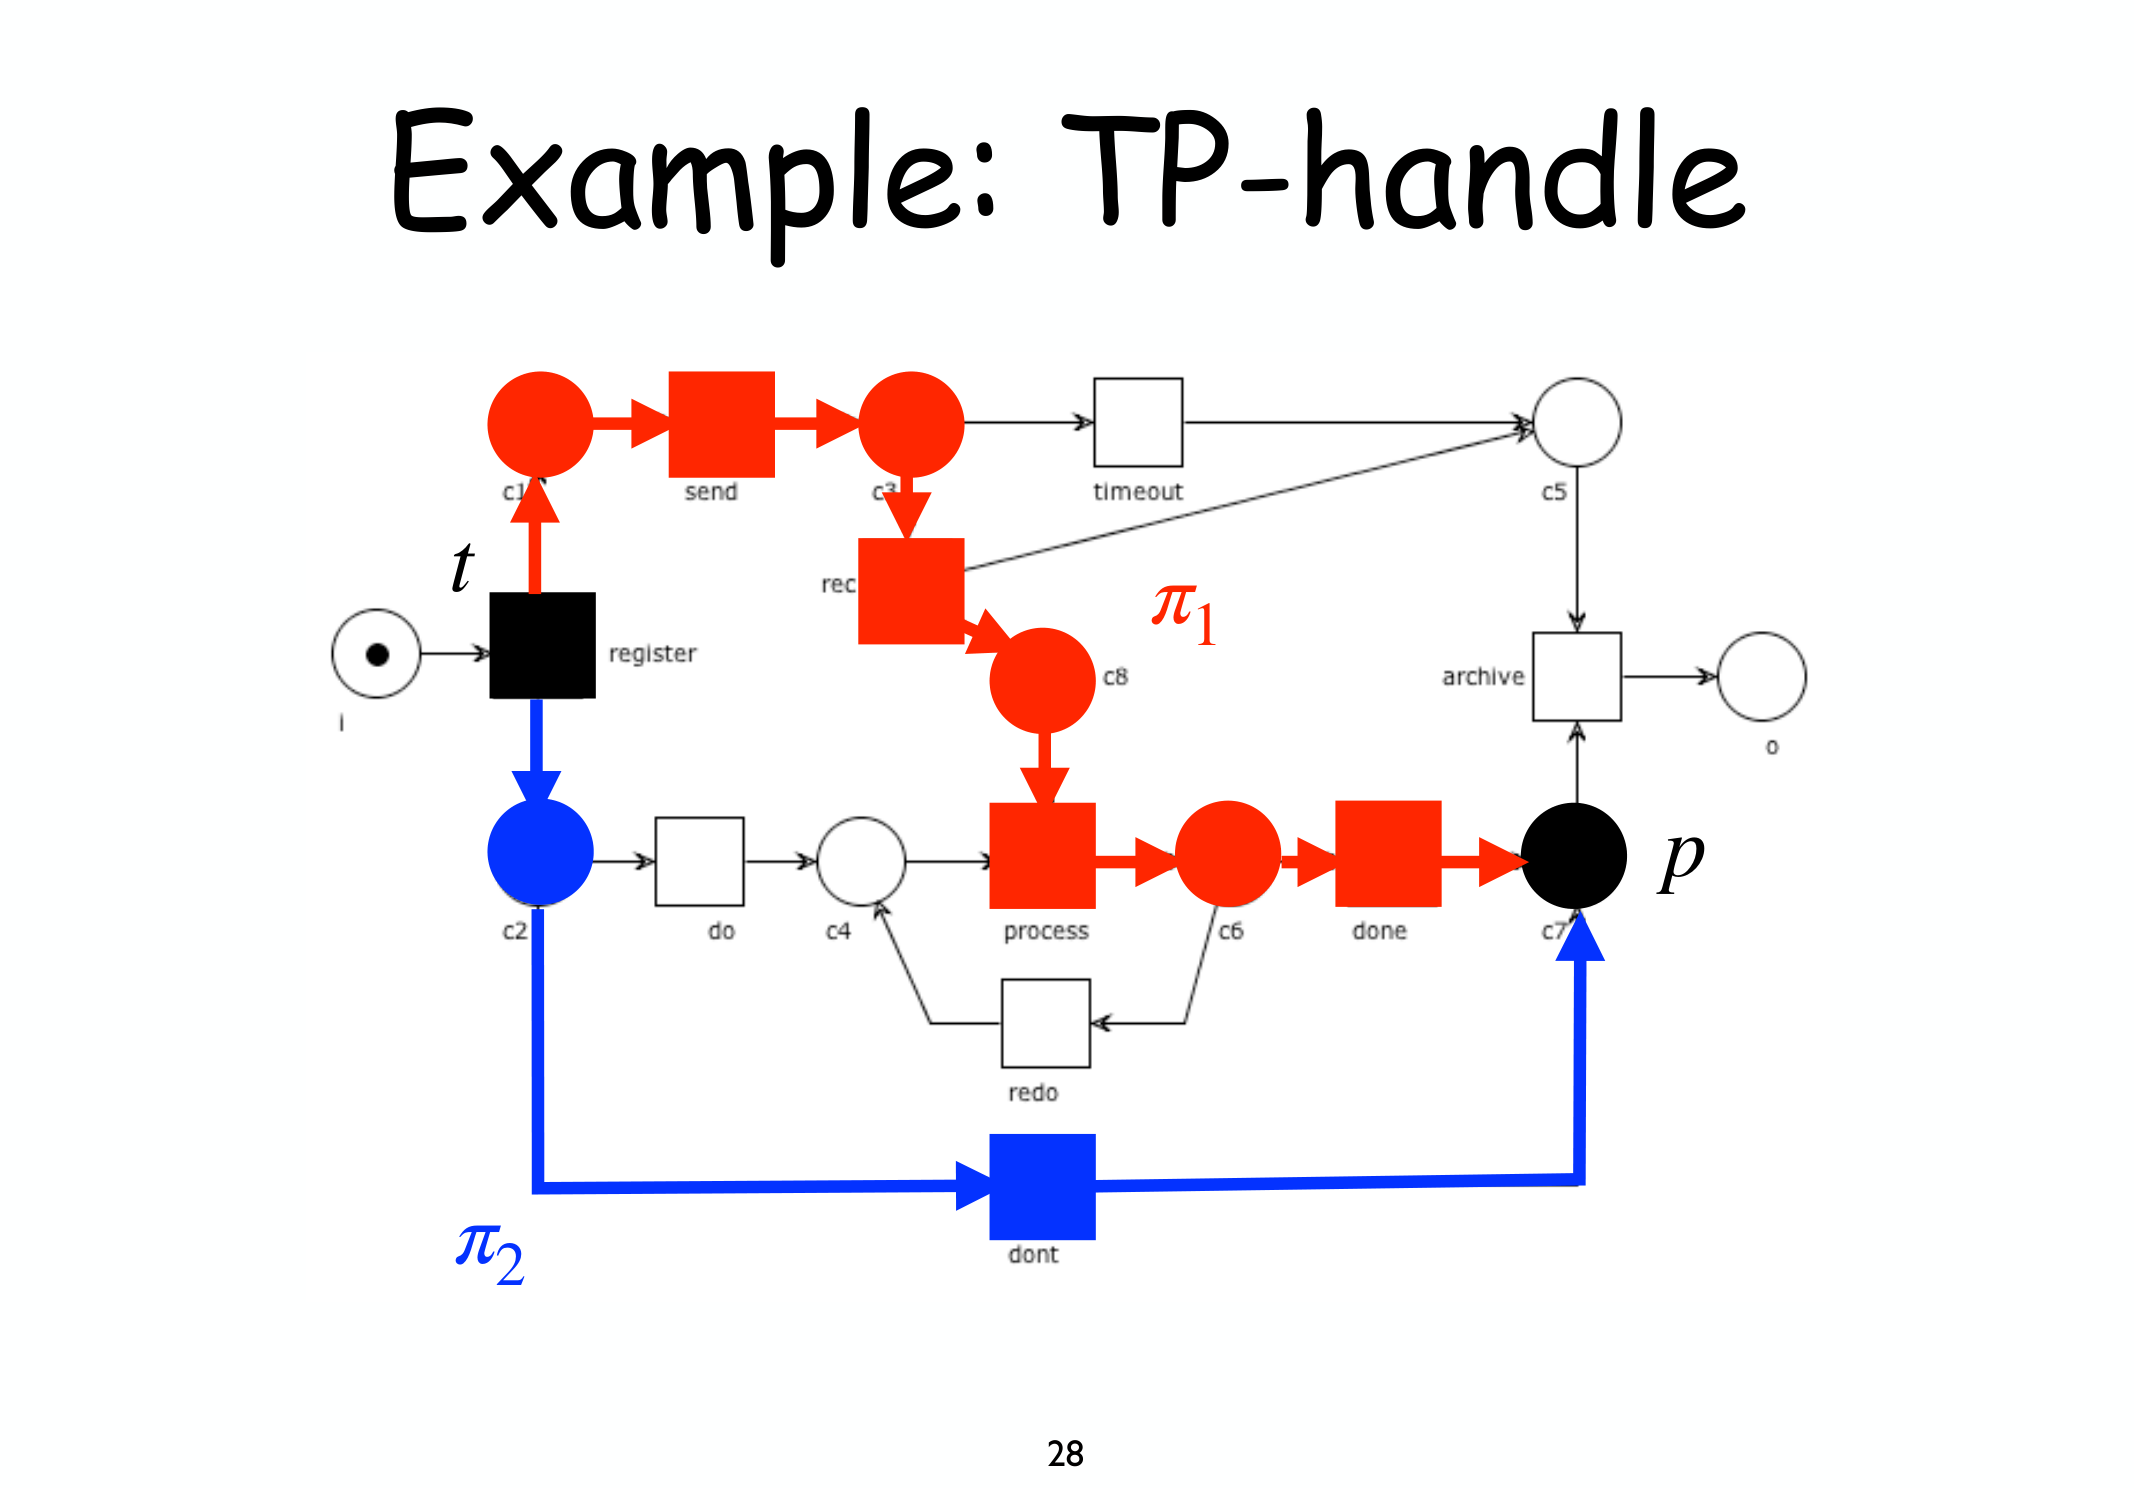
\includegraphics[width=0.74\linewidth,height=0.34\textheight,keepaspectratio]{images/21-wfnets-diagnosis_p28_tp-handle.png}
\caption{Un TP-handle: due cammini paralleli da \texttt{register} (AND-split, $t$) confluiscono nello stesso place $p$ senza una vera sincronizzazione — sintomo tipico di un \textbf{AND-split seguito da un XOR-join}, che può produrre token multipli.}
\end{figure}

Il difetto duale riguarda l'ordine opposto: uno XOR-split i cui rami vengono poi \textbf{sincronizzati} come se fossero paralleli.

\begin{boxdefinition}{PT-handle}
Un place $p$ e una transizione $t$ formano un \textbf{PT-handle} se esistono due cammini elementari distinti $\pi_1,\pi_2$ da $p$ a $t$ con soli $p,t$ in comune.

Il caso tipico è uno \textbf{XOR-split} ($p$) i cui due rami alternativi vengono poi sincronizzati da un \textbf{AND-join} ($t$): siccome i due rami sono \textbf{mutuamente esclusivi}, l'AND-join aspetterà per sempre il ramo non scelto — \textbf{deadlock}.
\end{boxdefinition}

\begin{figure}[!htb]
\centering
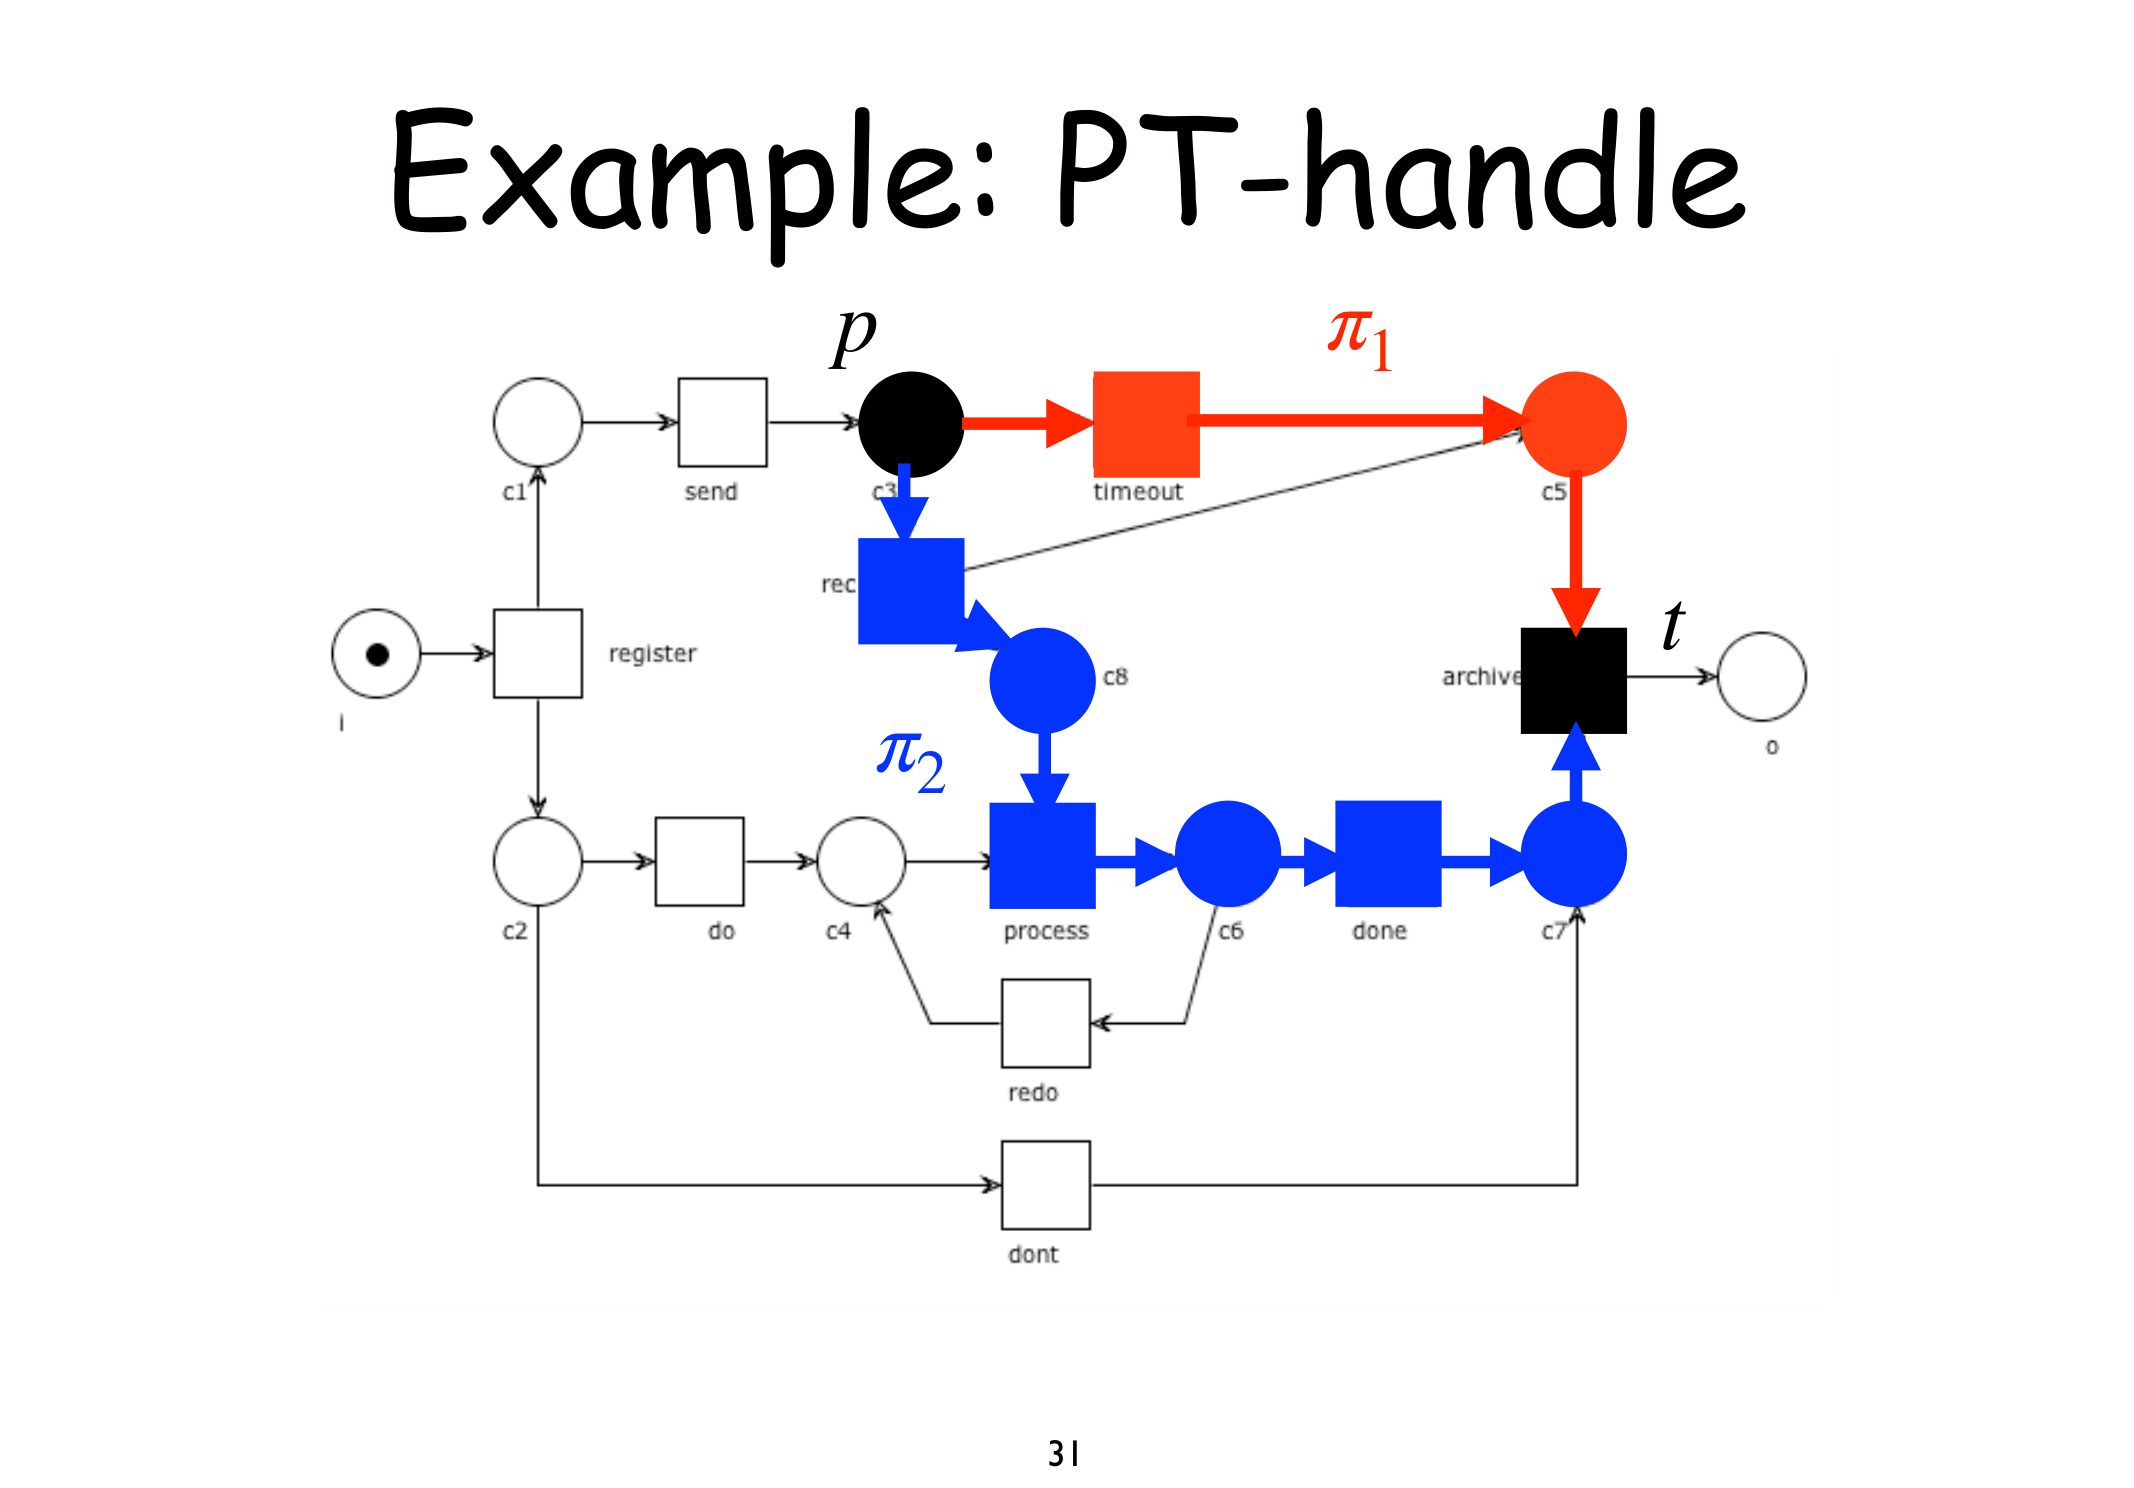
\includegraphics[width=0.74\linewidth,height=0.34\textheight,keepaspectratio]{images/21-wfnets-diagnosis_p31_pt-handle.png}
\caption{Un PT-handle: due cammini da $p$ (c3, uno XOR-split implicito) a $t$ (\texttt{archive}) condividono solo gli estremi — se i due rami sono in realtà \textbf{alternativi}, la sincronizzazione in $t$ può bloccarsi in attesa del ramo scartato.}
\end{figure}

\begin{boxdefinition}{Well-handled e well-structured}
Una rete è \textbf{well-handled} se \textbf{non} ha né TP-handle né PT-handle. Un workflow net $N$ è \textbf{well-structured} se $N^\star$ è well-handled.
\end{boxdefinition}

\begin{boxtheorem}{S-coverability theorem 2}
Se $N$ è \textbf{sound} e \textbf{well-structured}, allora $N^\star$ è \textbf{S-coverable}.

\textbf{Conseguenza pratica} (contronominale):

\[
N \text{ well-structured} \ \wedge\ N^\star \text{ non S-coverable} \ \Rightarrow\ N \text{ non è sound}
\]

Anche qui, come per il teorema 1, WoPeD calcola gli handle su $N^\star$ (reset implicito), non su $N$.
\end{boxtheorem}

\section{\texorpdfstring{Error sequences: individuare lo scenario minimo del difetto}{Error sequences: individuare lo scenario minimo del difetto}}

I due criteri precedenti sono \textbf{strutturali}: dicono che qualcosa non va, ma non sempre indicano \emph{la sequenza di eventi} che porta al problema. Le \textbf{error sequence} colmano questo buco: sono le \textbf{scene del crimine} più brevi possibili.

\begin{boxdefinition}{Error sequence (idea generale)}
Una error sequence è una firing sequence tale che: 1. \textbf{ogni continuazione} porta a un errore (option to complete o proper completion violate); 2. è \textbf{minimale}: nessun prefisso proprio ha già questa proprietà.

Cattura l'essenza dell'errore di design nel modo più compatto possibile — uno "scenario minimo" da mostrare al progettista.
\end{boxdefinition}

Le due varianti corrispondono ai due modi di rompere la soundness: la liveness (option to complete) e la boundedness (proper completion).

\subsection{\texorpdfstring{Non-live sequences}{Non-live sequences}}

\begin{boxdefinition}{Non-live sequence}
Una \textbf{non-live sequence} è una firing sequence più corta possibile dopo la quale \textbf{completare il caso non è più possibile} — cioè un testimone del fatto che la transizione \textbf{reset} è non-live in $N^\star$.
\end{boxdefinition}

\begin{boxtheorem}{Proprietà fondamentale}
Se $N^\star$ è \textbf{bounded} e $N$ \textbf{non ha task dead}, allora:

\[
N^\star \text{ è live} \quad\iff\quad N \text{ non ha non-live sequence}
\]
\end{boxtheorem}

L'analisi è possibile solo su sistemi \textbf{bounded} (altrimenti il reachability graph non è nemmeno finito) e si visualizza colorando gli stati del RG:

\begin{boxnote}{Colorazione del reachability graph}
\begin{itemize}
\item \textbf{verde}: da questo stato, \textbf{ogni} cammino porta a $o$ (tutto bene);
\item \textbf{rosso}: da questo stato, \textbf{nessun} cammino porta a $o$ (condannato);
\item \textbf{giallo}: \textbf{alcuni} cammini portano a $o$, altri no (ancora recuperabile, ma rischioso).
\end{itemize}

Le non-live sequence sono i cammini più corti che portano da uno stato giallo a uno \textbf{rosso}.
\end{boxnote}

\begin{figure}[!htb]
\centering
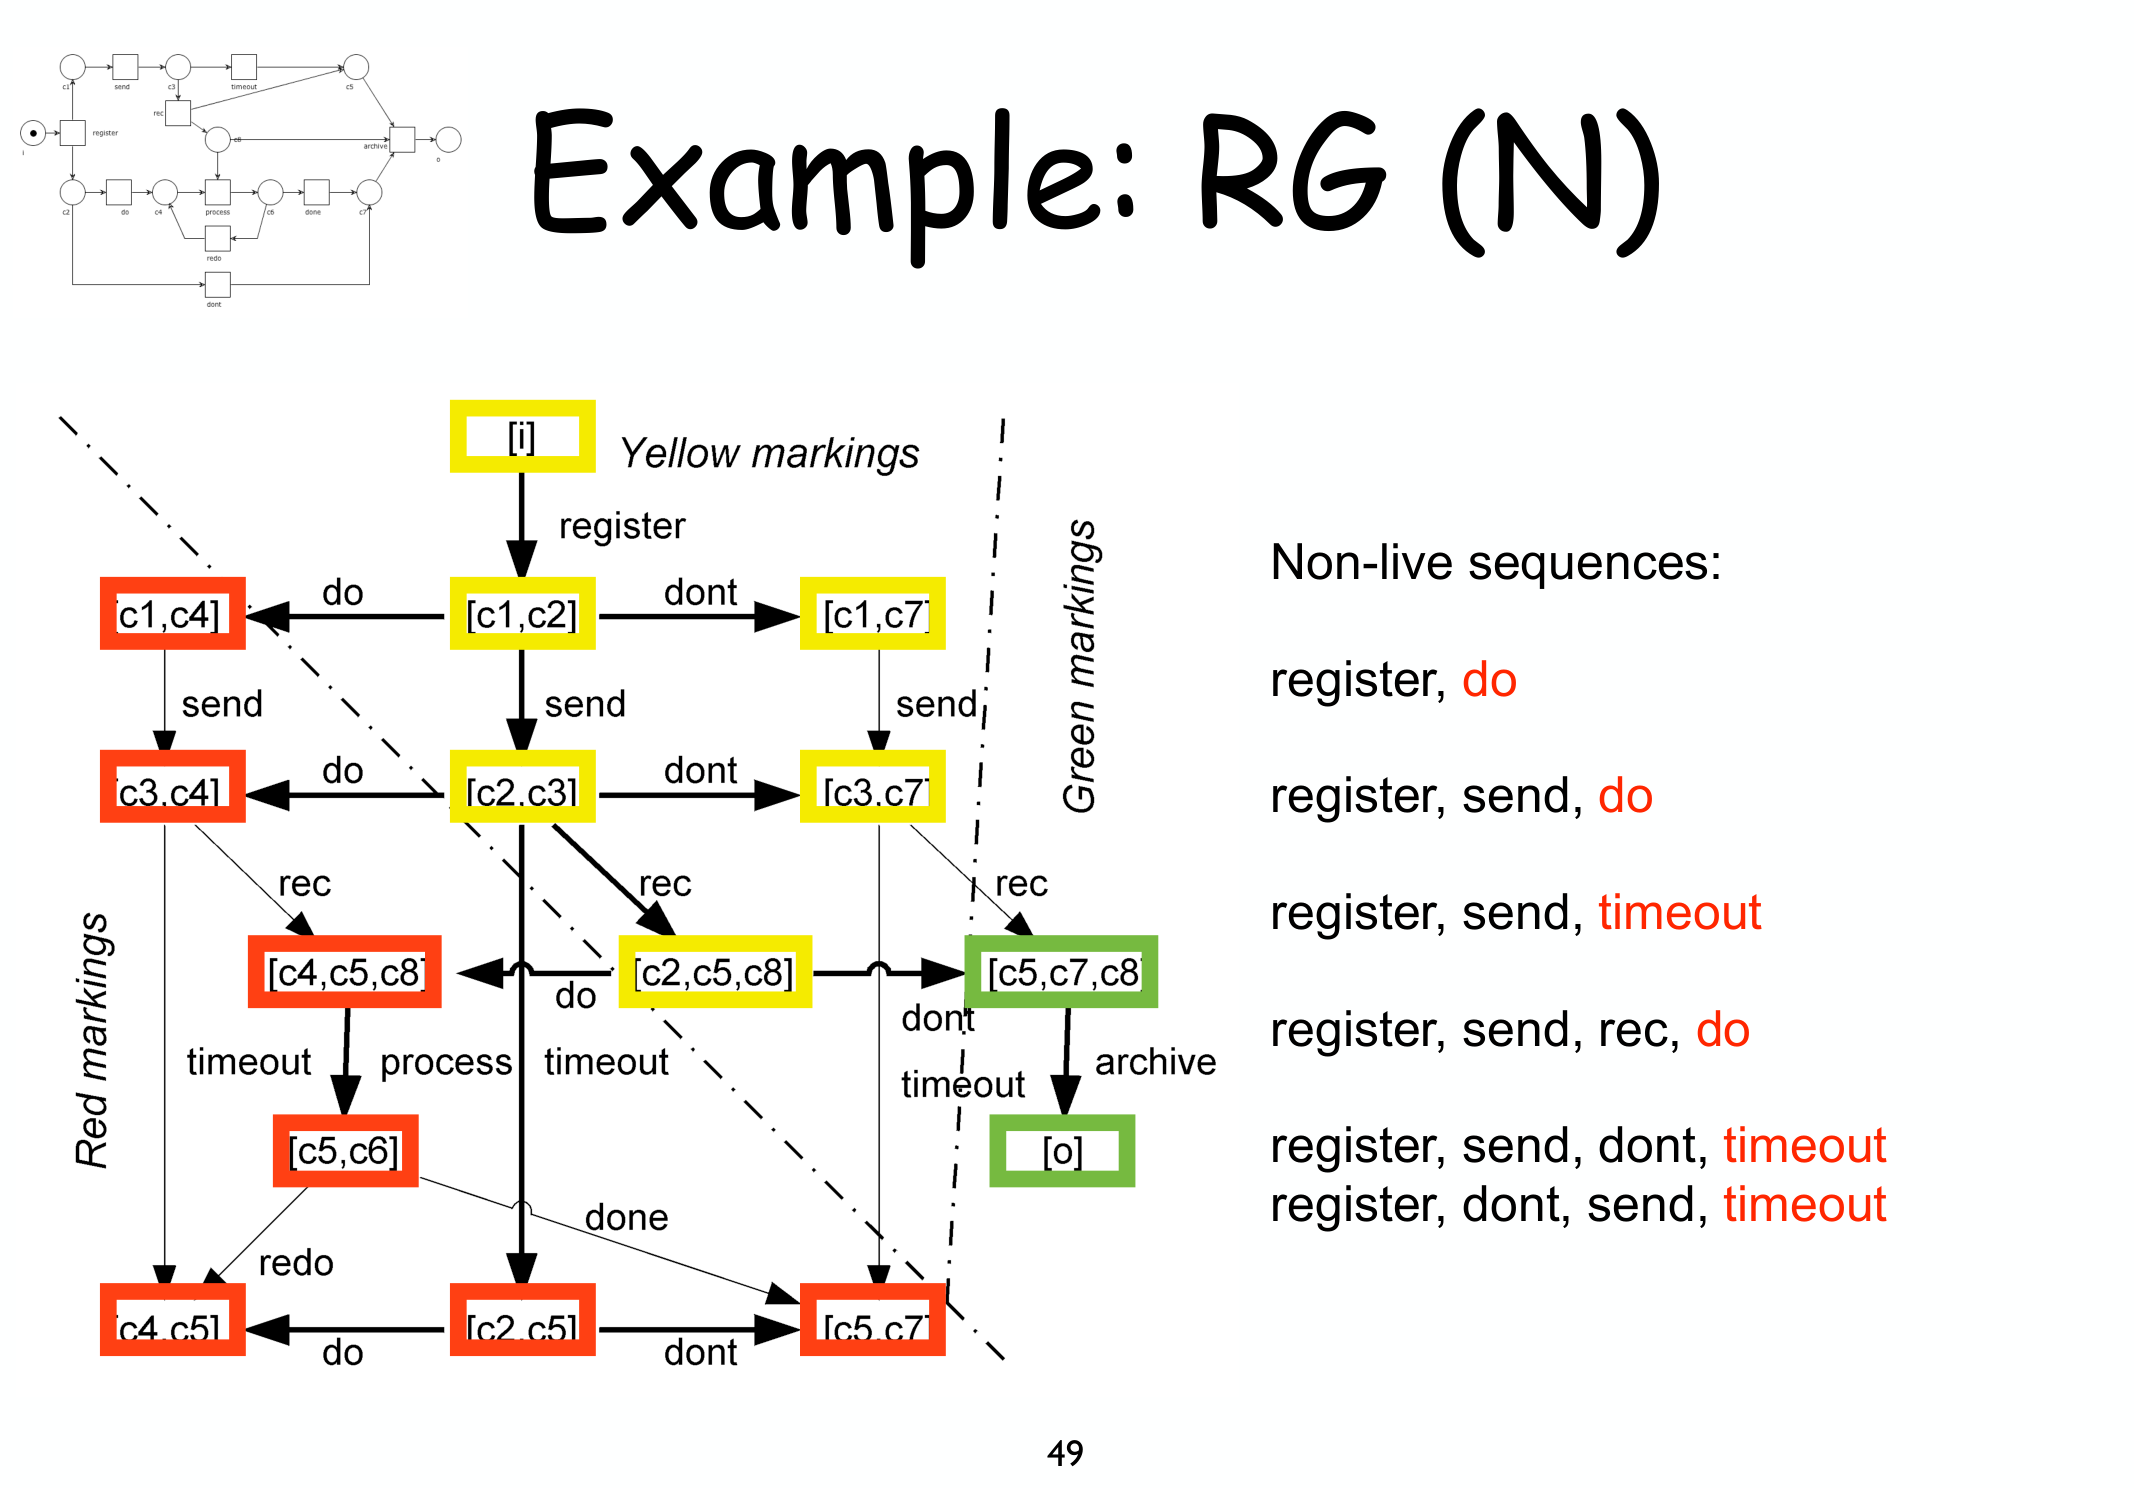
\includegraphics[width=0.74\linewidth,height=0.34\textheight,keepaspectratio]{images/21-wfnets-diagnosis_p49_rg-nonlive.png}
\caption{Il reachability graph colorato: dagli stati \textbf{gialli} (ancora recuperabili) alcuni scatti portano al \textbf{verde} (\texttt{[o]}, tutto bene) e altri al \textbf{rosso} (condannato). Le non-live sequence — \texttt{register,do}; \texttt{register,send,do}; \texttt{register,send,timeout}; … — sono gli scenari \textbf{più corti} che finiscono nel rosso: mostrano al progettista esattamente quale sequenza di scelte porta al blocco.}
\end{figure}

\subsection{\texorpdfstring{Unbounded sequences}{Unbounded sequences}}

Il difetto duale riguarda la boundedness: invece di bloccarsi, la rete potrebbe accumulare \textbf{infiniti token}.

\begin{boxdefinition}{Unbounded sequence}
Una \textbf{unbounded sequence} è una firing sequence di lunghezza minima tale che \textbf{ogni continuazione invalida la proper completion} — un testimone dell'unboundedness. Le marcature "indesiderate" sono quelle con peso infinito o quelle \textbf{strettamente maggiori} di $o$ (token in eccesso oltre al solo place finale).
\end{boxdefinition}

\begin{boxtheorem}{Proprietà fondamentale}
\[
N^\star \text{ è bounded} \quad\iff\quad N \text{ non ha unbounded sequence}
\]
\end{boxtheorem}

La visualizzazione usa lo stesso schema a tre colori, ma sul \textbf{coverability graph} (CG, che rappresenta anche le marcature "infinite" con un simbolo $\omega$):

\begin{boxnote}{Colorazione del coverability graph}
\begin{itemize}
\item \textbf{verde}: da qui le marcature indesiderate \textbf{non sono raggiungibili};
\item \textbf{rosso}: da qui \textbf{nessuna} marcatura verde è raggiungibile (le indesiderate sono inevitabili);
\item \textbf{giallo}: le indesiderate sono raggiungibili ma \textbf{evitabili}.
\end{itemize}
\end{boxnote}

Poiché il CG può diventare enorme (ogni marcatura $\omega$ genera altre marcature $\omega$, tutte rosse), conviene evitare di espanderle: nasce così una versione più economica.

\begin{boxtip}{Restricted Coverability Graph (RCG)}
Osservazione chiave: una marcatura a peso infinito genera \textbf{solo altre} marcature a peso infinito, e saranno \textbf{tutte rosse}. Si può quindi evitare del tutto di calcolarle, marcando direttamente come rosso il nodo che le genererebbe — risparmiando gran parte dell'esplorazione senza perdere informazione utile.
\end{boxtip}

\begin{figure}[!htb]
\centering
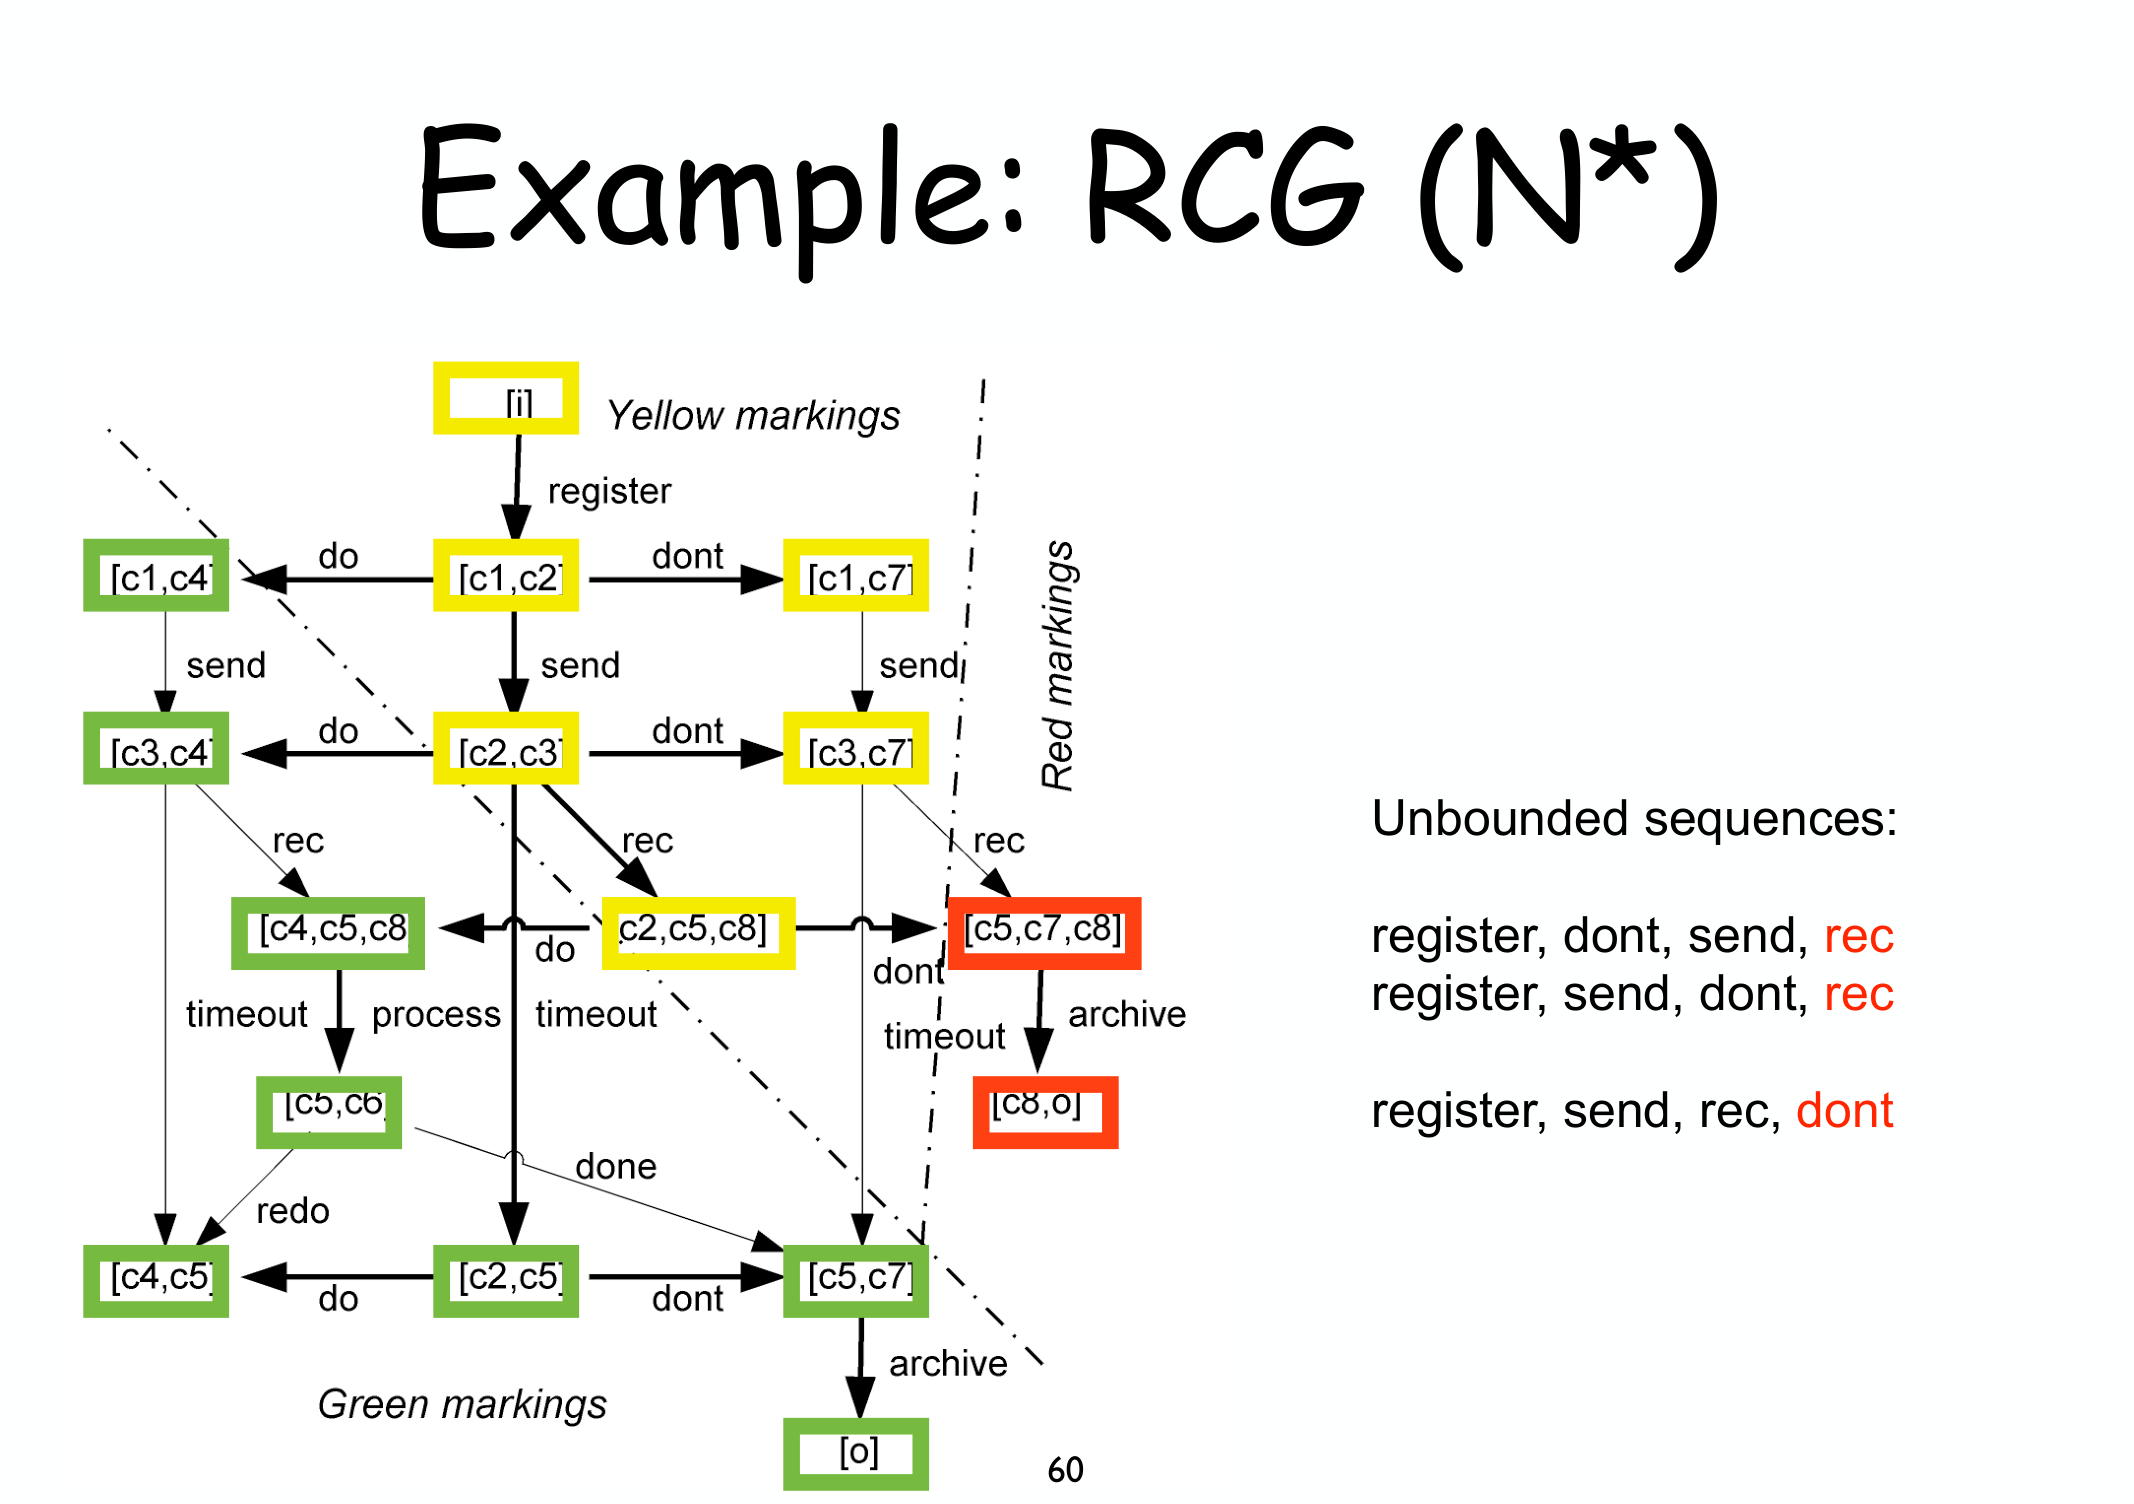
\includegraphics[width=0.74\linewidth,height=0.34\textheight,keepaspectratio]{images/21-wfnets-diagnosis_p60_rcg-unbounded.png}
\caption{L'RCG evita di espandere gli stati a peso infinito (subito rossi), riducendo drasticamente lo spazio esplorato. Le unbounded sequence — es. \texttt{register,send,rec,dont} — sono gli scenari minimi che portano a un accumulo di token.}
\end{figure}

\section{\texorpdfstring{Woflan e ProM: gli strumenti in pratica}{Woflan e ProM: gli strumenti in pratica}}

Questi criteri sono implementati in tool reali, pensati per dare diagnosi utilizzabili senza dover leggere a mano il reachability graph.

\begin{boxnote}{Woflan (WOrkFLow ANalyzer)}
Verifica se $N$ è un sound workflow net rispondendo a tre domande in sequenza: \emph{è $N$ un workflow net?} \emph{è $N^\star$ bounded?} \emph{è $N^\star$ live?} In caso negativo, fornisce diagnostica (place unbounded, transizioni dead o non-live). Nato come tool standalone per Windows, oggi è un \textbf{plugin di ProM} (promtools.org).
\end{boxnote}

\begin{boxwarning}{Il limite della diagnostica "a insiemi"}
Sapere \emph{quali} place sono unbounded o \emph{quali} transizioni sono dead è utile ma spesso \textbf{non basta} a capire la causa esatta dell'errore. Le \textbf{error sequence} (sopra) sono il complemento che localizza il problema in uno \textbf{scenario concreto}, invece che in un insieme statico di nodi sospetti.
\end{boxwarning}

\section{\texorpdfstring{Chiusura del corso}{Chiusura del corso}}

Con questa lezione si chiude il percorso su Petri net e workflow: dalla costruzione (\hyperref[ch:04]{04 — Petri Nets}) alla verifica strutturale (S/T-system, free-choice), dalla soundness alla sua \textbf{diagnosi pratica}. Il messaggio finale del corso, esplicito nelle ultime slide, è che quanto visto è solo \textbf{la punta dell'iceberg} del Business Process Management: dietro restano ancora notazione, teoria, tecnologia, strumenti, metodologia, encoding, validazione e verifica — un intero campo di ricerca sotto la superficie, lasciato all'esplorazione di chi vuole andare oltre.